% Options for packages loaded elsewhere
\PassOptionsToPackage{unicode}{hyperref}
\PassOptionsToPackage{hyphens}{url}
\PassOptionsToPackage{dvipsnames,svgnames,x11names}{xcolor}
%
\documentclass[
  authoryear,
  preprint]{elsarticle}

\usepackage{amsmath,amssymb}
\usepackage{iftex}
\ifPDFTeX
  \usepackage[T1]{fontenc}
  \usepackage[utf8]{inputenc}
  \usepackage{textcomp} % provide euro and other symbols
\else % if luatex or xetex
  \usepackage{unicode-math}
  \defaultfontfeatures{Scale=MatchLowercase}
  \defaultfontfeatures[\rmfamily]{Ligatures=TeX,Scale=1}
\fi
\usepackage{lmodern}
\ifPDFTeX\else  
    % xetex/luatex font selection
\fi
% Use upquote if available, for straight quotes in verbatim environments
\IfFileExists{upquote.sty}{\usepackage{upquote}}{}
\IfFileExists{microtype.sty}{% use microtype if available
  \usepackage[]{microtype}
  \UseMicrotypeSet[protrusion]{basicmath} % disable protrusion for tt fonts
}{}
\makeatletter
\@ifundefined{KOMAClassName}{% if non-KOMA class
  \IfFileExists{parskip.sty}{%
    \usepackage{parskip}
  }{% else
    \setlength{\parindent}{0pt}
    \setlength{\parskip}{6pt plus 2pt minus 1pt}}
}{% if KOMA class
  \KOMAoptions{parskip=half}}
\makeatother
\usepackage{xcolor}
\setlength{\emergencystretch}{3em} % prevent overfull lines
\setcounter{secnumdepth}{5}
% Make \paragraph and \subparagraph free-standing
\makeatletter
\ifx\paragraph\undefined\else
  \let\oldparagraph\paragraph
  \renewcommand{\paragraph}{
    \@ifstar
      \xxxParagraphStar
      \xxxParagraphNoStar
  }
  \newcommand{\xxxParagraphStar}[1]{\oldparagraph*{#1}\mbox{}}
  \newcommand{\xxxParagraphNoStar}[1]{\oldparagraph{#1}\mbox{}}
\fi
\ifx\subparagraph\undefined\else
  \let\oldsubparagraph\subparagraph
  \renewcommand{\subparagraph}{
    \@ifstar
      \xxxSubParagraphStar
      \xxxSubParagraphNoStar
  }
  \newcommand{\xxxSubParagraphStar}[1]{\oldsubparagraph*{#1}\mbox{}}
  \newcommand{\xxxSubParagraphNoStar}[1]{\oldsubparagraph{#1}\mbox{}}
\fi
\makeatother


\providecommand{\tightlist}{%
  \setlength{\itemsep}{0pt}\setlength{\parskip}{0pt}}\usepackage{longtable,booktabs,array}
\usepackage{calc} % for calculating minipage widths
% Correct order of tables after \paragraph or \subparagraph
\usepackage{etoolbox}
\makeatletter
\patchcmd\longtable{\par}{\if@noskipsec\mbox{}\fi\par}{}{}
\makeatother
% Allow footnotes in longtable head/foot
\IfFileExists{footnotehyper.sty}{\usepackage{footnotehyper}}{\usepackage{footnote}}
\makesavenoteenv{longtable}
\usepackage{graphicx}
\makeatletter
\def\maxwidth{\ifdim\Gin@nat@width>\linewidth\linewidth\else\Gin@nat@width\fi}
\def\maxheight{\ifdim\Gin@nat@height>\textheight\textheight\else\Gin@nat@height\fi}
\makeatother
% Scale images if necessary, so that they will not overflow the page
% margins by default, and it is still possible to overwrite the defaults
% using explicit options in \includegraphics[width, height, ...]{}
\setkeys{Gin}{width=\maxwidth,height=\maxheight,keepaspectratio}
% Set default figure placement to htbp
\makeatletter
\def\fps@figure{htbp}
\makeatother

\makeatletter
\@ifpackageloaded{caption}{}{\usepackage{caption}}
\AtBeginDocument{%
\ifdefined\contentsname
  \renewcommand*\contentsname{Table of contents}
\else
  \newcommand\contentsname{Table of contents}
\fi
\ifdefined\listfigurename
  \renewcommand*\listfigurename{List of Figures}
\else
  \newcommand\listfigurename{List of Figures}
\fi
\ifdefined\listtablename
  \renewcommand*\listtablename{List of Tables}
\else
  \newcommand\listtablename{List of Tables}
\fi
\ifdefined\figurename
  \renewcommand*\figurename{Figure}
\else
  \newcommand\figurename{Figure}
\fi
\ifdefined\tablename
  \renewcommand*\tablename{Table}
\else
  \newcommand\tablename{Table}
\fi
}
\@ifpackageloaded{float}{}{\usepackage{float}}
\floatstyle{ruled}
\@ifundefined{c@chapter}{\newfloat{codelisting}{h}{lop}}{\newfloat{codelisting}{h}{lop}[chapter]}
\floatname{codelisting}{Listing}
\newcommand*\listoflistings{\listof{codelisting}{List of Listings}}
\makeatother
\makeatletter
\makeatother
\makeatletter
\@ifpackageloaded{caption}{}{\usepackage{caption}}
\@ifpackageloaded{subcaption}{}{\usepackage{subcaption}}
\makeatother
\journal{Journal Name}

\ifLuaTeX
  \usepackage{selnolig}  % disable illegal ligatures
\fi
\usepackage[]{natbib}
\bibliographystyle{elsarticle-harv}
\usepackage{bookmark}

\IfFileExists{xurl.sty}{\usepackage{xurl}}{} % add URL line breaks if available
\urlstyle{same} % disable monospaced font for URLs
\hypersetup{
  pdftitle={Towards Next Generation Risk Assessment of PFAS. Development and evaluation of a mechanistic human PBK model for PFOA.},
  pdfauthor={Chrysanthi Pachoulide; Joost Westerhout; Nynke I. Kramer},
  pdfkeywords={PFOA, Physiologically Based Kinetic
modelling, read-across, Global Sensitivity Analysis, Next Generation
Risk Assessment},
  colorlinks=true,
  linkcolor={blue},
  filecolor={Maroon},
  citecolor={Blue},
  urlcolor={Blue},
  pdfcreator={LaTeX via pandoc}}


\setlength{\parindent}{6pt}
\begin{document}

\begin{frontmatter}
\title{Towards Next Generation Risk Assessment of PFAS. Development and
evaluation of a mechanistic human PBK model for PFOA. \\\large{Step 1} }
\author[1]{Chrysanthi Pachoulide%
\corref{cor1}%
\fnref{fn1}}
 \ead{chrysanthi.pachouide@wur.nl} 
\author[2]{Joost Westerhout%
%
\fnref{fn2}}
 \ead{joost.westerhout@rivm.nl} 
\author[1]{Nynke I. Kramer%
%
\fnref{fn3}}
 \ead{nynke.kramer@wur.nl} 

\affiliation[1]{organization={Wageningen University and
Research, Division of Toxicology},addressline={Stippeneng
4},city={Wageningen},postcode={6708 WE},postcodesep={}}
\affiliation[2]{organization={RIVM, Department Name},addressline={Street
Address},city={Utrecht},postcode={Postal Code},postcodesep={}}

\cortext[cor1]{Corresponding author}
\fntext[fn1]{This is the first author footnote.}
\fntext[fn2]{Another author footnote, this is a very long footnote and
it should be a really long footnote. But this footnote is not yet
sufficiently long enough to make two lines of footnote text.}
\fntext[fn3]{Yet another author footnote.}
        
\begin{abstract}
Per- and polyfluoroalkyl substances (PFAS) represent a substantial
chemical class, comprising thousands of structurally diverse chemicals,
which only have in common one fully fluorinated methyl or methylene
carbon atom. PFAS are ubiquitous environmental pollutants of
anthropogenic nature and therefore of potential risk to human health.
Human toxicological risk assessment of PFAS is challenging, due to their
sheer number, structural diversity and paucity of the relevant data
required to identify and characterize them. A solution to this challenge
lies in the application of read-across approach, which involves the
extrapolation of information from a data-rich PFAS to make predictions
about a similar data-poor one. One example of this approach could be the
application of a Physiologically Based Kinetic (PBK) model from PFOA, to
inform the development of PBK models for PFASs with analogous
physicochemical properties. Despite the availability of several PBK
models for PFOA, all of them rely on PFOA-specific animal-sourced data
and are optimised to correctly predict the long half-lives observed in
humans. This hinders their use in the read-across scope, where PBK
models should be as mechanistic as possible, with key toxicokinetic
processes are described based on either in vitro or in silico studies.
The present study introduces a human mechanistic PBK model for PFOA,
that uses only in vitro derived input parameters. The uptake and
elimination of PFOA are predicted using in vitro to in vivo
extrapolation principles, while its tissue distribution is predicted
using experimentally derived distribution coefficients to tissue
components, such as albumin and phospholipids. The model introduces a
minimal mechanistic kidney compartment to predict the active
re-absorption of PFOA in the proximal tubules and a mechanistic
transporter-mediated entero-hepatic circulation. Furthermore, given the
high affinity of PFOA to albumin, the unbound fraction determined in
plasma, is adjusted to the differential albumin concentration between
the plasma and tissue or tubular fluid compartments, to better describe
an albumin facilitated transport of PFOA. The predicted Area Under the
Curve (AUC) and half-life were compared to the concentration over time
curve from a human volunteer study as well as to observed plasma
concentrations and half-lives from the latest human biomonitoring data.
Finally, the Global Sensitivity Analysis (GSA) workflow recommended by
the OECD PBK guideline was applied to both evaluate the validity of the
model and inform about the key parameters determining the PBK model
predictions. The newly developed PFOA PBK model can be extrapolated to
other PFASs for which these key parameters are already available. The
subsequent derivation of these parameters for other PFASs will
facilitate the extrapolation of the present PBK models to them as well
and enable their human toxicological risk assessment.
\end{abstract}





\begin{keyword}
    PFOA \sep Physiologically Based Kinetic
modelling \sep read-across \sep Global Sensitivity Analysis \sep 
    Next Generation Risk Assessment
\end{keyword}
\end{frontmatter}
    

\section{Introduction}\label{introduction}

Per- and polyfluoroalkyl substances (PFAS) represent a substantial
chemical class, comprising thousands of structurally diverse chemicals,
which only have in common one fully fluorinated methyl or methylene
carbon atom. PFAS are ubiquitous environmental pollutants of
anthropogenic nature and therefore of potential risk to human health.
Human toxicological risk assessment of PFAS is challenging, due to their
sheer number, structural diversity and paucity of the relevant data
required to identify and characterize them. A solution to this challenge
lies in the application of read-across approach, which involves the
extrapolation of information from a data-rich PFAS to make predictions
about a similar data-poor one. One example of this approach could be the
application of a Physiologically Based Kinetic (PBK) model from PFOA, to
inform the development of PBK models for PFASs with analogous
physicochemical properties. Despite the availability of several PBK
models for PFOA, all of them rely on PFOA-specific animal-sourced data
and are optimised to correctly predict the long half-lives observed in
humans. This hinders their use in the read-across scope, where PBK
models should be as mechanistic as possible, with key toxicokinetic
processes are described based on either in vitro or in silico studies.
The present study introduces a human mechanistic PBK model for PFOA,
that uses only in vitro derived input parameters.

Too many PFAS PFOA toxicokinetic understanding long half-life,
persistence strong binding to proteins (especially albumin and
fatty-acid binding proteins) and membrane phospholipids Discussion about
previous PBK approaches, need of fitting to data \& use of parameters
taken from animal studies - read-across not possible - What we need:
more generic, that we can use for PFAS for which we don't know
information

\section{Materials and Methods}\label{materials-and-methods}

\subsection{PBK Model Development}\label{pbk-model-development}

The PFOA human PBK model was developed with the aim of being as minimal
and mechanistic as possible for read-across in a NGRA framework. For
this, the critical toxicokinetic processes relevant for PFAS were
included, those being renal elimination and re-absorption, enterohepatic
circulation and oral, dermal or inhalation exposure. The model was
evaluated against observed \emph{in vivo} concentration-time profiles in
plasma as well as observed half-life in humans, from human biomonitoring
data.\footnote{Could consider also evaluation against urine and fecal
  concentrations from Abraham study, but in this study they mentioned
  that urinary PFOA concentrations were contaminated while fecal
  concentrations (ng/g feces) don't represent fecal daily excretion and
  can't be used for data evaluation}

\subsubsection{Model structure}\label{model-structure}

The PBK model was build on the model previously used by EFSA and
recently updated to include dermal exposure \citep{husøy2023}. The model
was updated to include physiological processes related to renal
elimination and re-absorption, as well as enterohepatic circulation. The
model structure included the intestinal, kidney and liver compartments
which are responsible for the above-mentioned toxicokinetic processes
and the option to include skin and lungs in case relevant exposure
routes are used.

\paragraph{Absorption}\label{absorption}

\subparagraph{Oral absorption}\label{oral-absorption}

Oral absorption via food or drinks is the main route of exposure to
PFOA. PFOA is quickly and efficiently absorbed from the
gastro-intestinal tract to portal circulation
\citep{abraham2024}\footnote{Plasma Tmax of 2h after oral exposure (from
  Abraham)}. A most physiological and mechanistic model for the
gastro-intestinal tract (GIT) was initially considered to fully describe
the toxicokinetic process involved in the absorption and elimination of
PFOA in that organ. PFOA could be absorbed in all sections of the GIT
both by passive diffusion of the fraction non-ionised and active uptake
of the fraction ionised at the pH of the corresponding section. Uptake
via both passive and active processes has been also observed in \emph{in
vitro} uptake studies \citep{kimura2017, janssen2024} . The initial
model subdivided the GIT into the stomach, upper small intestine
(duodenum and jejunum), lower small intestine (ileum) and large
intestine. Each intestinal sub-section was further divided into the
lumen and intestinal vascular tissue. Absorption of PFOA was modelled as
an uptake clearance from the lumen to the intestinal tissue, while the
fraction of PFOA that was not absorbed in each section was transferred
to the following section, or eliminated to the faeces, based on
physiological transit times \citep{willmann2004}. In the final model,
the GIT was simplified to only one compartment as the initial more
complex model did not significantly altered the absorption profile of
PFOA\footnote{Insert reference to predictions in supplementary material}.

\subparagraph{Dermal absorption}\label{dermal-absorption}

Dermal absorption can occur after exposure via cosmetic products or dust
disposed on skin. Dermal absorption was modelled using a
compartmentalised skin compartment with a separate skin barrier
(epidermis) and rest of skin compartment. Absorption of PFOA from the
skin barrier was defined as the absorption clearance\footnote{Is it
  correct to call it a clearance? I perceive clearance as an elimination
  parameter, but I could be wrong.}, while once PFOA was in the rest of
skin compartment it was then distributed to the systemic plasma
concentration.

\subparagraph[Inhalation absorption]{\texorpdfstring{Inhalation
absorption\footnote{tentative\ldots{}}}{Inhalation absorption}}\label{inhalation-absorption5}

Fast absorption, with Tmax at 3h post exposure (rats)
\citep{gustafsson2022}

PFAS delivery on lung surfactants facilitated by albumin
\citep{forsthuber2020}

For air partition coef \citep{yao2025}

\subsubsection{Distribution}\label{distribution}

Tissue distribution of PFOA was assumed to be perfusion limited, as not
enough mechanistic data is available to support a permeability limited
model. Permeability limited PBK models for PFOA have been already
developed, but they under-predict plasma concentrations and require the
addition of a fitted parameter to correctly describe a reabsorption
process from cells to plasma \citep{lin2023, cheng2017}. In previous
PFOA PBK models, tissue-plasma partition coefficients were determined
from \emph{in vivo} animal steady-state tissue and plasma
concentrations. This approach has been recently proven not adequate due
to significant inter-species variabilities in the toxicokinetics of
PFOA\footnote{refer to Deepika/Annelies study}. An alternative approach
to defining tissue-plasma partition coefficients, is the mechanistic
tissue-plasma partition algorithms, that use physiochemical properties
(such as the octanol-water partition coefficient Kow and acid
disociation constant pKa) to predict the chemical affinities tissue
components (proteins or lipids), assuming that these depend on the
lipophilicity and ionisation status of the chemical. The final
steady-state tissue-plasma distribution is based on the differences in
composition of the different tissues and their respective volume
\citep{Rodgers2007, Utsey2020b, Peyret2010}. However, these algorithms
are limited to the chemical-space for which they have been validated for
and cannot be applied to PFAS. PFAS, due to their amphiphilic nature lie
outside of the applicability domain of these algorithms as they don't
have a Kow. Recently, the binding affinity of PFOA to different tissue
components (membrane phospholipids, storage lipids, structural proteins,
albumin, fatty-acid binding protein) was derived experimentally
\citep{allendorf2020}. PFOA showed high affinity for albumin, fatty acid
binding proteins and membrane phospholipids, while it's binding affinity
to structural proteins and storage lipids was lower. Tissue-plasma
partition coefficients were calculated using the above mentioned
distribution coefficients. Physiological data about the relevant tissue
components were taken from literature \citep{allendorf2020, utsey2020}.
To enable comparison of the calculated partition coefficients with the
previously used \emph{in vivo} derived ones, partition coefficients were
derived for both rat and human tissues. Results are available in
supplementary file\ldots{}

\subsubsection{Elimination}\label{elimination}

Renal and biliary elimination of PFOA has been well documented, while
renal and intestinal reabsorption are believed to be the mechanisms
determining its long plasma half-life.

\paragraph{Renal elimination}\label{renal-elimination}

Multiple mechanisms can be involved in the renal elimination of PFOA,
including glomerular filtration, active tubular secretion and
re-absorption and passive permeability. Several studies have showed that
PFOA is a substrate of organic anion transporters, while recently its
intrinsic clearance by these transporters was determined in vitro, using
either HEK293, or CHO cells transfected with the specific transporter
\citep{yang2010, janssen2024, ryu2024, lin2023}. PFOA can be actively
secreted from the plasma to the proximal tubule cells by OAT1 and OAT3
transporters and actively re-absorbed from the primary urine to the
proximal tubule cells by OAT4 and URAT1 transporters
\citep{yang2010, janssen2024, ryu2024, lin2023}. The available
un-ionised PFOA can also freely diffuse between plasma, cells and the
primary urine. A mechanistic kidney was developed, based on models
previously developed for drugs undergoing renal reabsorption
\citep{scotcher2016, huang2018, pletz2021}. Briefly, the proximal tubule
was explicitly modelled as local PFOA concentrations are determining the
extend of transporter mediated re-absorption. All other kidney sections
(loop of Henle, distal tube and the collecting duct) were lumped
together as rest-of-kidney as it was assumed that they don't
significantly contribute to PFOA renal kinetics. Each section was
initially sub-divided to plasma, cellular and luminar sub-sections where
PFOA is distributed based on the active and or passive processes
mentioned above. In the final model, the plasma and cellular
compartments were lumped together to as active secretion by OAT1 and
OAT3 transporters did not significantly contribute to the model
predictions, while passive re-absorption from the proximal tubule cell
to the plasma was not enough to accurately predict plasma
concentrations, leading to PFOA accumulation in the proximal tubule
cells\footnote{Not sure if I should further elaborate on this.}.

\paragraph{Enterohepatic circulation}\label{enterohepatic-circulation}

\subsection{Model parametrization}\label{model-parametrization}

The uptake and elimination of PFOA are predicted using in vitro to in
vivo extrapolation principles, while its tissue distribution is
predicted using experimentally derived distribution coefficients to
tissue components, such as albumin and phospholipids. The model
introduces a minimal mechanistic kidney compartment to predict the
active re-absorption of PFOA in the proximal tubules and a mechanistic
transporter-mediated entero-hepatic circulation. Furthermore, given the
high affinity of PFOA to albumin, the unbound fraction determined in
plasma, is adjusted to the differential albumin concentration between
the plasma and tissue or tubular fluid compartments, to better describe
an albumin facilitated transport of PFOA.

\subsubsection{Derivation of partition
coefficients}\label{derivation-of-partition-coefficients}

\subsubsection{In Vitro to In Vivo
extrapolation}\label{in-vitro-to-in-vivo-extrapolation}

\subsubsection{Prediction of the adjusted-fraction
unbound}\label{prediction-of-the-adjusted-fraction-unbound}

\subsection{Model evaluation}\label{model-evaluation}

\subsubsection{Global Sensitivity Analysis
Workflow}\label{global-sensitivity-analysis-workflow}

\paragraph{Morris screaning test}\label{morris-screaning-test}

\paragraph{eFAST test}\label{efast-test}

\subsubsection{Evaluation against human biomonitoring
data}\label{evaluation-against-human-biomonitoring-data}

Check this study
\citep{domingo2025, convertino2018, hanvoravongchai2024, botelho2025, lin2024, faquih2024}

\section{Results}\label{results}

\subsection{Model development}\label{model-development}

Think if the results of the tissue-plasma partition coefficients are
needed here. I think its enough to have them in the supplementary data.

Model figure Show results with \& without sub compartments, from most
complex to less complex and which processess were included

\subsection{Model evaluation}\label{model-evaluation-1}

\subsubsection{Global Sensitivity
Analysis}\label{global-sensitivity-analysis}

Finally, the Global Sensitivity Analysis (GSA) workflow recommended by
the OECD PBK guideline was applied to both evaluate the validity of the
model and inform about the key parameters determining the PBK model
predictions.

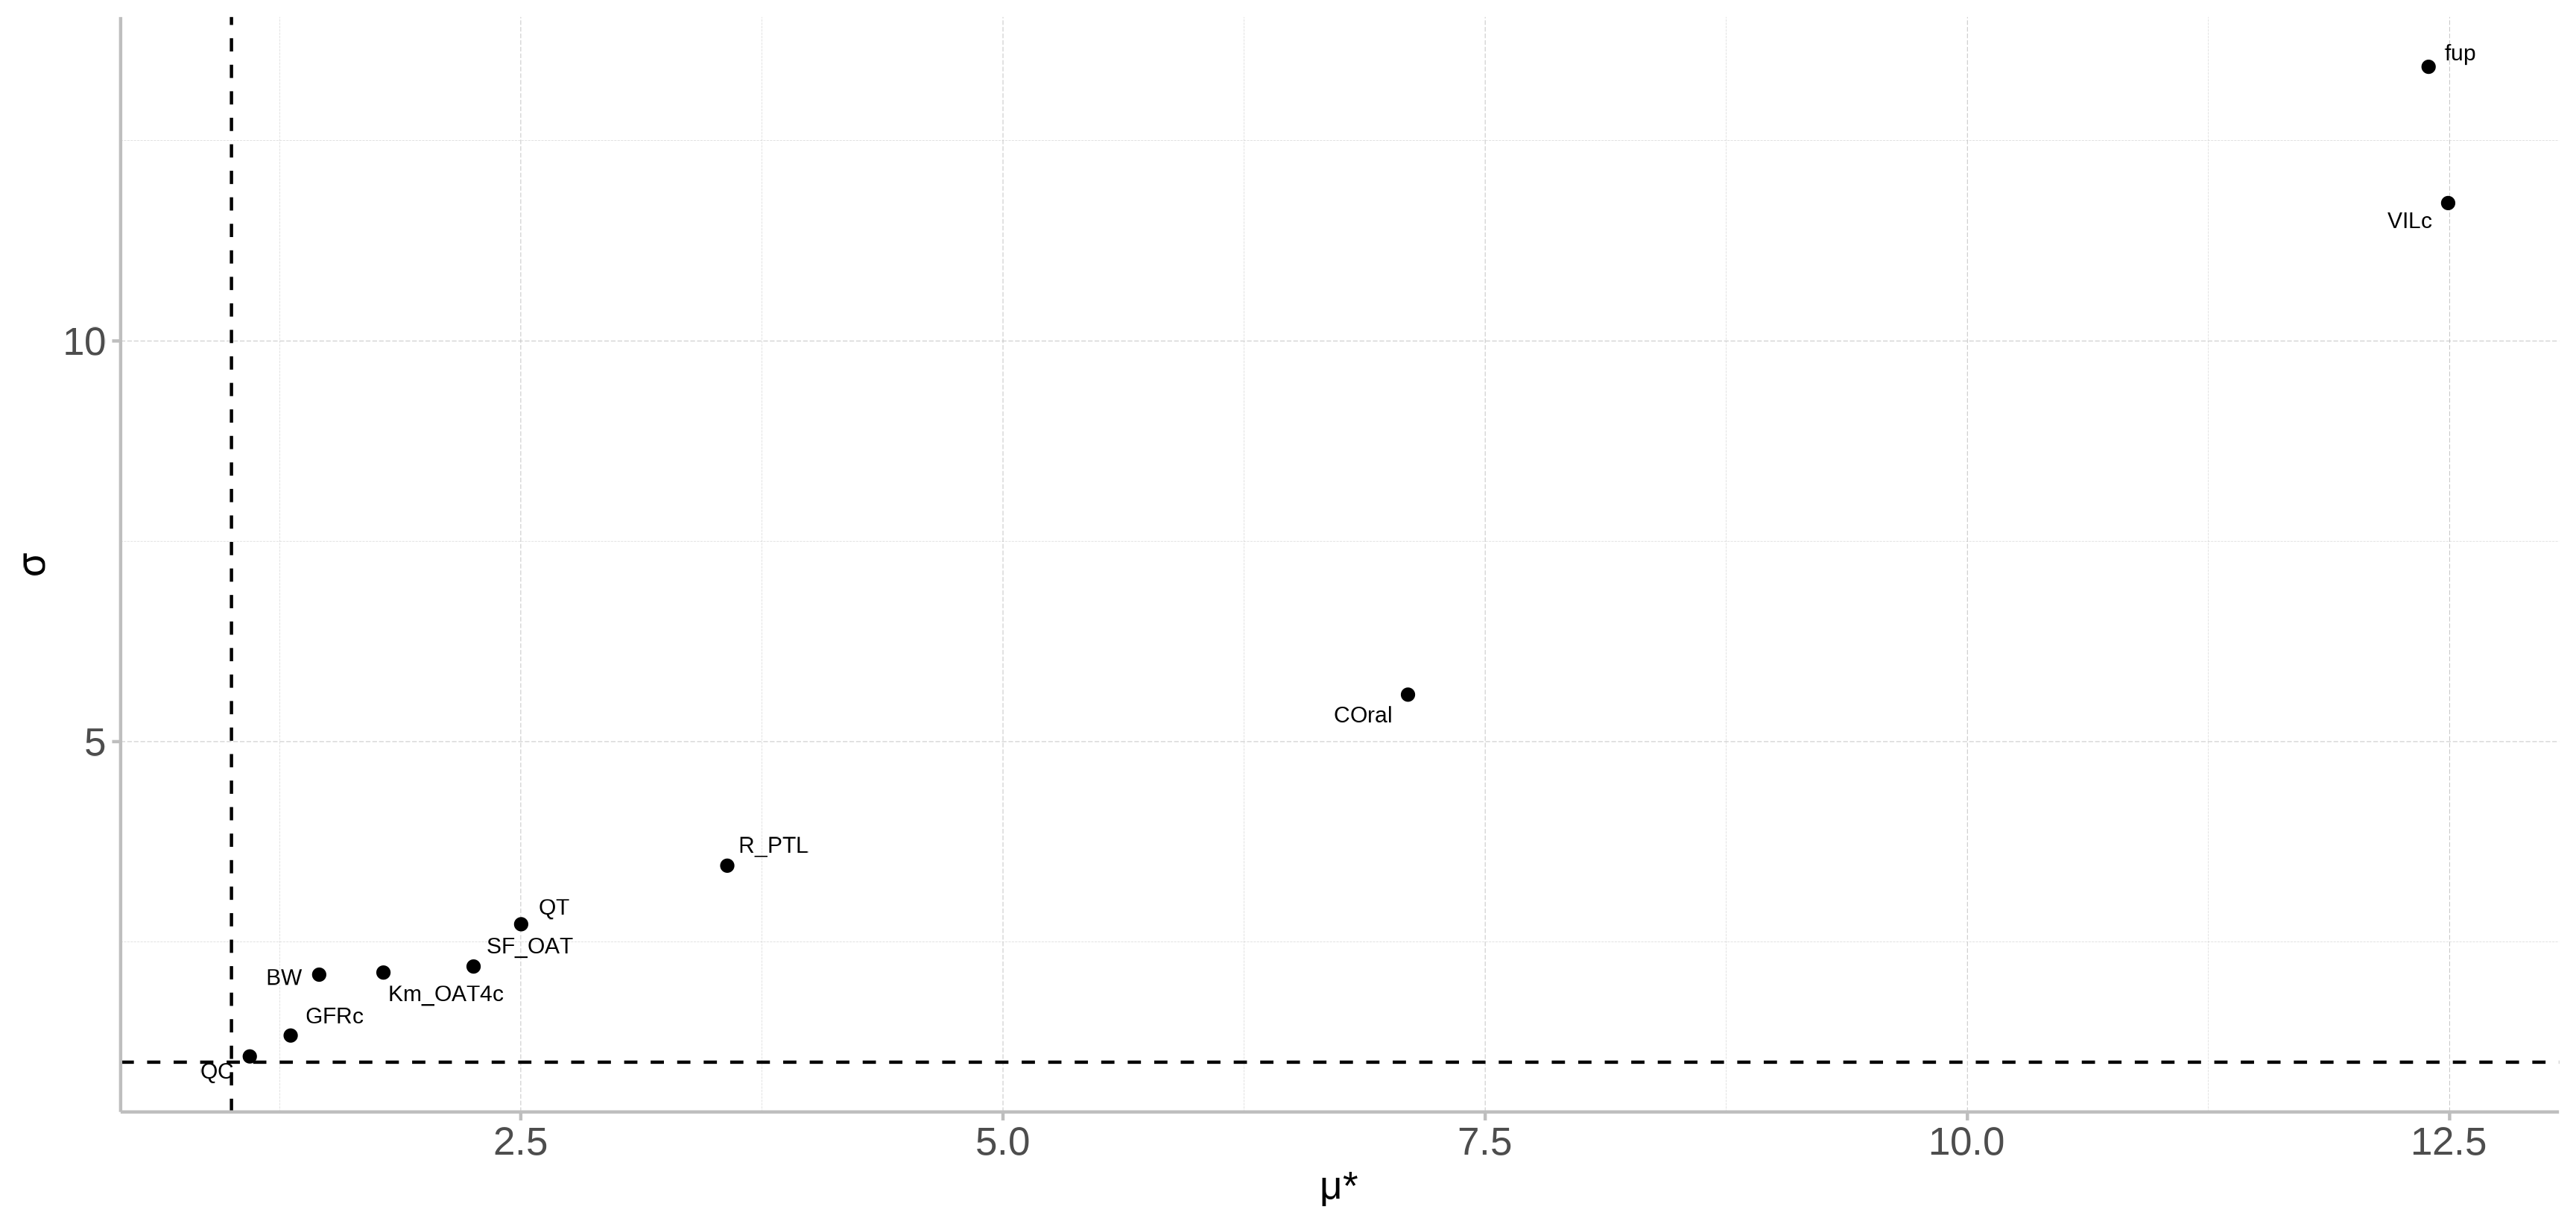
\includegraphics{images/MorrisResultNocolour.plot.png}

\subsubsection{Evaluation against human biomonitoring
data}\label{evaluation-against-human-biomonitoring-data-1}

The predicted Area Under the Curve (AUC) and half-life were compared to
the concentration over time curve from a human volunteer study as well
as to observed plasma concentrations and half-lives from the latest
human biomonitoring data.

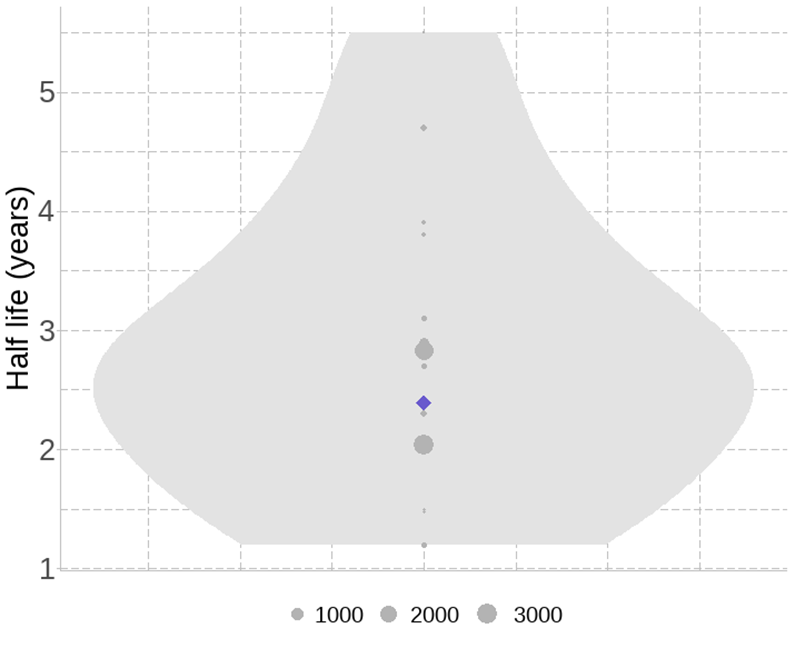
\includegraphics{images/clipboard-3078347208.png}

\section{Discussion}\label{discussion}

Oral absorption/GIT: differential absorption of PFOA in the GIT
depending on it's ionisation status could have been significant if we
separately considered passive absorption of the non-ionised form and
active absorption of the non-ionised form. But we couldn't do it as
mechanistic data on this is not available.

Model limitations : tissue absorption not fully understood, uncertainty
of the most sensitive parameters Potential uses?!

The newly developed PFOA PBK model can be extrapolated to other PFASs
for which these key parameters are already available. The subsequent
derivation of these parameters for other PFASs will facilitate the
extrapolation of the present PBK models to them as well and enable their
human toxicological risk assessment.

Distribution: Recently, equilibrium tissue distribution coefficients
were derived using PFOA tissue concentrations found in healthy human
forensic autopsies of different tissues. This approach could be
considered more physiologically relevant, however its application would
increase the uncertainty of the model some limitations were the sizes of
the tissue samples, that might not be representative of the whole tissue
concentrations, as well as the variability in blood compositions due to
blood coagulation in some of the samples. \citep{baumert2023}

Distribution: the need of a fitted parameter in permeability limited
models suggest a rapid equilibrium of PFOA concentrations in plasma and
cells.

Finally passive processes could be important in determining the half
life of PFOA in specific populations, such as patients with chronic
kidney disease (CKD), which has actually been linked to PFOA exposure.
CKD leads to decreased GFR and changes in urinary pH, both of which
alter the passive permeability of PFOA in the kidney \citep{huang2018} .
This is interesting to model, especially for the assessment of the risk
of PFOA exposure in that population.

\section{Conclusion}\label{conclusion}

\section{Funding}\label{funding}

\section{CRediT authorship contribution
statement}\label{credit-authorship-contribution-statement}

\section{Declaration of Competing
Interest}\label{declaration-of-competing-interest}

\section{Acknowledgement}\label{acknowledgement}

\section{Appendix A. Supporting
information}\label{appendix-a.-supporting-information}

\section{Data availability}\label{data-availability}


\renewcommand\refname{References}
  \bibliography{bibliography.bib}



\end{document}
